\documentclass[pdf]{beamer}
%\usetheme{CambridgeUS}
\usetheme{Warsaw}
\usepackage{bbm}
\usepackage{apacite}
\usepackage[english]{babel}
\usepackage{amssymb,amsthm,makeidx,verbatim,latexsym,amsfonts,graphicx,mathrsfs}
\usepackage{nomencl,tikz,caption,subcaption,enumitem,multicol,natbib,bm,lscape}
\usepackage{tasks,comment,url,float,pdfpages,tabularx,booktabs,longtable}
%\usepackage[hidelinks]{hyperref}
%\usepackage[tbtags]{amsmath}
\usepackage{colortbl,multirow,mathtools}
\usetikzlibrary{shapes.multipart}
\usetikzlibrary{positioning,calc,shapes.geometric,arrows,matrix,fit,backgrounds,intersections}
\makenomenclature
\setbeamercovered{transparent}
%\useoutertheme[subsection=false]{smoothbars}
\useinnertheme{rectangles}

\mode<presentation>{}
%% preamble
\title{MACHINE LEARNING WITH APPLICATIONS IN AGRICULTURE}
%\subtitle[short version]{A subtitle}
\date[2021]{FEBRUARY, 2021}
\author[ABIODUN ALLISON]{\textbf{ABIODUN UTHMAN ALLISON \texorpdfstring{\\ MATRIC NO: 204603}{}}}
\institute{\textbf{A M.Sc. RESEARCH PROJECT SUBMITTED TO THE
DEPARTMENT OF MATHEMATICS, FACULTY OF SCIENCE,
UNIVERSITY OF IBADAN, IBADAN, NIGERIA.}\\ \vskip 0.3cm
\textbf{SUPERVISOR: PROF. G.O.S. EKHAGUERE}}
%%completed


\begin{document}
\frame{\maketitle} % <-- generate frame with title

\begin{frame}{TABLE OF CONTENTS}
\tableofcontents
\end{frame}


\section{Introduction}
\begin{frame}[allowframebreaks]{Introduction}
\small
Agriculture could be referred to as the production, processing, promotion and distribution of agricultural products. It plays a critical role in the economy of developing countries. Besides supplying food and raw materials, agriculture also provides the populace with job opportunities. \\
The Food and Agriculture Organization of the United Nations (FAO) estimates that pests and diseases lead to the loss of $20 - 40 \%$ of global food production, constituting a threat to food security (Food and Agriculture Organization of the United Nation, International Plant Protection Convention, 2017). \\
Machine learning is the scientific study of algorithms and mathematical models that computer systems use to perform a specific task without using explicit instructions, relying on patterns and inference instead. It is a branch of Artificial Intelligence (AI) focused on the premise that, with minimal human interaction, systems can learn from data, recognize trends and make decisions. In supervised machine learning, a training set of $D$ input  vectors $\{\bm{x}_1, \bm{x}_2, \hdots , \bm{x}_D\}$ is used to tune the parameters of an adaptive model, along with their corresponding target vectors $\bm{y}$, in order to accurately predict vector $\hat{\bm{y}}$. We focus on a subset of supervised learning, called classification, where the aim is to assign each input vector to one of a finite number of discrete categories \\
Computer vision, and object recognition in particular, has made tremendous advances in the past few years. In 2012, a large, deep convolutional neural network achieved a top-5 test error (the fraction of test images for which the correct label is not among the five labels considered most probable by the model) rate of $15.3\ \%$, at the Large Scale Visual Recognition Challenge (ILSVRC) 2012 image classification competition for the classification of $15$ million images into $22$ thousand possible categories \textbf{~\cite{Krizhevsky}}. 
\end{frame}


\section{Literature Review}
\begin{frame}[allowframebreaks]{Literature Review}
\small
\textbf{Johnson and Stulz, 1987} was the first paper covering default risk in options. They considered many options with writer's default risk which are written by private financial institutions that have limited assets instead of organized exchanges and there are no guarantee by a third party. Therefore, they assumed that if the option writer is unable to make a promised payment, the vulnerable option holders receive all the assets of the option writer. They derived closed form solutions for the European option prices in some different cases by assuming stochastic processes both for the asset value of the option writer and the value of the underlying asset.\\
\textbf{Zhou and Li, 2019} considered the pricing problem of options with counterparty default risks. They studied the asymptotic behaviour of vulnerable option prices under an uncertain volatility model which contains both corporate assets and underlying assets. They presented an estimation method for solving a fully non-linear P.D.E by imposing additional conditions to the boundary conditions and substituted it into two Black-Scholes like equations whereby they obtained a method to estimate the price of vulnerable options in the worst case scenario.
\end{frame}
\normalsize
\section{Pricing of Options with Default Risks under The First Passage Time Model}

\small
\begin{frame}[allowframebreaks]{Theorem}
%\begin{theorem}
Assume $B_{1}(t), B_{2}(t)$ are correlated Brownian motions with drift terms $\alpha t, \beta t$ and $d B_{1}(t) d B_{2}(t)= \rho dt$. Then
\small
\[
\begin{aligned}
&\int_{\bar{b}_{2}}^{\infty} \int_{\bar{b}_{1}}^{\infty} \int_{\bar{m}_{1}}^{\infty} e^{p b_{1}+q b_{2}} f_{M_{1}(T), B_{1}(T), B_{2}(T)}(m_{1}, b_{1}, b_{2}) d m_{1} d b_{1} d b_{2} \\
&=e^{T(\frac{p^{2}}{2}+\rho p q+\frac{q^{2}}{2}+\alpha p+\beta q)}\\
&N_{2}\bigg(-\frac{\bar{b}_{1}}{\sqrt{T}}+\sqrt{T}(\alpha+p+\rho q),-\frac{\bar{b}_{2}}{\sqrt{T}}+\sqrt{T}(\beta+\rho p+q), \rho\bigg) \\
&-e^{T(\frac{p^{2}}{2}+\rho p q+\frac{q^{2}}{2}+\alpha p+\beta q)+2 \bar{m}_{1}(p+\rho q)+2 \alpha \bar{m}_{1}}\\
& N_{2}\bigg(-\frac{\bar{b}_{1}-2 \bar{m}_{1}}{\sqrt{T}}+\sqrt{T}(\alpha+p+\rho q),-\frac{\bar{b}_{2}-2 \rho \bar{m}_{1}}{\sqrt{T}}+\sqrt{T}(\beta+\rho p+q), \rho \bigg)
\end{aligned}
\]
where $N_{2}(u, v, \rho)$ is the cumulative distribution function of a bivariate standard normal distribution defined by
$$
N_{2}(u, v, \rho) \equiv \int_{-\infty}^{v} \int_{-\infty}^{u} \frac{1}{2 \pi \sqrt{1-\rho^{2}}} e^{-\frac{1}{2(1-\rho^{2})}(x^{2}-2 \rho x y+y^{2})} d x d y
$$
\end{frame}
\begin{frame}[allowframebreaks]
Substituting $\bar{b}_{1} = d, \bar{b}_{2} = k, \bar{m}_{1} = l,\alpha = B_{1}(t), \beta =B_{2}(t)$, equation \eqref{eq:20} can be simplified with Theorem $1$ as follows:
\begin{equation}
\label{eq:33}
\begin{aligned} 
C &=(1-\delta) S_{0}\bigg[ N_{2}\bigg(-\frac{d}{\sqrt{T}}+\frac{\sqrt{T}}{\sigma_{v}}(r-\gamma-\frac{\sigma_{v}^{2}}{2}+\rho \sigma_{s} \sigma_{v}),\\
&-\frac{k}{\sqrt{T}}+\frac{\sqrt{T}}{\sigma_{s}}(r+\frac{\sigma_{s}^{2}}{2}), \rho \bigg)
\end{aligned}
\end{equation}
$$
\begin{aligned}
&- e^{2 \rho \sigma_{s} l+\frac{2 l}{\sigma_{v}}(r-\gamma-\frac{\sigma_{v}^{2}}{2})} N_{2}\bigg(\frac{2 l-d}{\sqrt{T}}+\frac{\sqrt{T}}{\sigma_{v}}(r-\gamma-\frac{\sigma_{v}^{2}}{2}+\rho \sigma_{s} \sigma_{v}),\\
& \frac{2 \rho l-k}{\sqrt{T}}+\frac{\sqrt{T}}{\sigma_{s}}(r+\frac{\sigma_{s}^{2}}{2}), \rho \bigg)\bigg]
\end{aligned}
$$
\begin{equation}
\label{eq:34}
\begin{aligned}
&- (1-\delta) K e^{-r T} \bigg[N_{2}(-\frac{d}{\sqrt{T}}+\frac{\sqrt{T}}{\sigma_{v}}(r-\gamma-\frac{\sigma_{v}^{2}}{2}),-\frac{k}{\sqrt{T}}+\frac{\sqrt{T}}{\sigma_{s}}(r-\frac{\sigma_{s}^{2}}{2}), \rho \bigg)
\end{aligned}
\end{equation}
$$
\begin{aligned}
&- e^{\frac{2 l}{\sigma_{v}}(r-\gamma-\frac{\sigma_{v}^{2}}{2})} N_{2}\bigg(\frac{2 l-d}{\sqrt{T}}+\frac{\sqrt{T}}{\sigma_{v}}(r-\gamma-\frac{\sigma_{v}^{2}}{2}), \frac{2 \rho l-k}{\sqrt{T}}+\frac{\sqrt{T}}{\sigma_{s}}(r-\frac{\sigma_{s}^{2}}{2}), \rho \bigg)\bigg]\\
&+ \delta (S_{0} N_{1} (d_{1})-K e^{-r T} N_{1}(d_{2}))
\end{aligned}
$$
Recall that
$$
\begin{aligned}
d_{1} = \frac{1}{\sigma_{s}\sqrt{T}}\ln \bigg[\frac{S_{0}e^{(r + \frac{\sigma_{s}^{2}}{2})T}}{K}\bigg],~~~~
d_{2} = \frac{1}{\sigma_{s}\sqrt{T}}\ln \bigg[\frac{S_{0}e^{(r - \frac{\sigma_{s}^{2}}{2})T}}{K}\bigg]
\end{aligned}
$$
Setting;
$$
\begin{aligned}
d_{3} = \frac{1}{\sigma_{v}\sqrt{T}}\ln \bigg[\frac{V_{0}e^{(r + \frac{\sigma_{v}^{2}}{2})T}}{D}\bigg],~~~~
d_{4} = \frac{1}{\sigma_{v}\sqrt{T}}\ln \bigg[\frac{V_{0}e^{(r - \frac{\sigma_{v}^{2}}{2})T}}{D}\bigg]
\end{aligned}
$$
By direct computation, $-\frac{k}{\sqrt{T}}+\frac{\sqrt{T}}{\sigma_{s}}(r+\frac{\sigma_{s}^{2}}{2})= d_{1}$ and $-\frac{d}{\sqrt{T}}+\frac{\sqrt{T}}{\sigma_{v}}(r-\gamma-\frac{\sigma_{v}^{2}}{2})=d_{4}$
\end{frame}
\normalsize
\begin{frame}[allowframebreaks]
Having obtained all the values, the pricing formula for a European call option with default risk is given by:
\begin{equation}
\label{eq:36}
\begin{aligned} 
C &=(1-\delta) S_{0}\bigg[N_{2}(d_{4}+\sqrt{T} \rho \sigma_{s}, d_{1}, \rho)\\
&- \underbrace{e^{2 \rho \sigma_{s} l + \frac{2 l}{\sigma_{v}}(r-\gamma-\frac{\sigma_{v}^{2}}{2})} N_{2}\bigg(d_{4}+ \frac{2 l}{\sqrt{T}} + \sqrt{T} \rho \sigma_{s}, d_{1}+ \frac{2 \rho l}{\sqrt{T}}, \rho \bigg)}_{A}\bigg] \\
&-(1-\delta) K e^{-r T}\bigg[N_{2}(d_{4}, d_{2}, \rho)\\
&- \underbrace{e^{\frac{2 l}{\sigma_{v}}(r-\gamma-\frac{\sigma_{v}^{2}}{2})} N_{2}\bigg(d_{4}+\frac{2 l}{\sqrt{T}}, d_{2}+ \frac{2 \rho l}{\sqrt{T}}, \rho \bigg)}_{B} \bigg] \\ 
&+\delta [S_{0} N_{1}(d_{1})-K e^{-r T} N_{1}(d_{2})]
\end{aligned}
\end{equation}
A European put option with default risk can also be evaluated by the aforementioned method. The analytical pricing formula is then given by:
\begin{equation}
\label{eq:37}
\begin{aligned} 
P &= (1-\delta) K e^{-r T}\bigg[N_{2}(d_{4}, -d_{2}, -\rho)- e^{\frac{2 l}{\sigma_{v}}(r-\gamma-\frac{\sigma_{v}^{2}}{2})}\\
& N_{2}\bigg(d_{4}+\frac{2 l}{\sqrt{T}}, -d_{2}- \frac{2 \rho l}{\sqrt{T}}, -\rho \bigg) \bigg] \\ 
&- (1-\delta) S_{0}\bigg[N_{2}(d_{4}+\sqrt{T} \rho \sigma_{s}, -d_{1}, -\rho)- e^{2 \rho \sigma_{s} l + \frac{2 l}{\sigma_{v}}(r-\gamma-\frac{\sigma_{v}^{2}}{2})}\\
& N_{2}\bigg(d_{4}+ \frac{2 l}{\sqrt{T}} + \sqrt{T} \rho \sigma_{s}, -d_{1}- \frac{2 \rho l}{\sqrt{T}}, -\rho \bigg)\bigg] \\
&+\delta [K e^{-r T} N_{1}(-d_{2}) - S_{0} N_{1}(-d_{1})]
\end{aligned}
\end{equation}
\end{frame}
\subsection{Reduction to Pricing of Options without Default Risks}
\begin{frame}[allowframebreaks]{Reduction to Pricing of Options without Default Risks}
The value of a European call option with default risk given in equation \eqref{eq:36} boils down to the Black-Scholes formula when the default risk of writer is ignored. Since the last term of equation \eqref{eq:36} is just $\delta$ times of Black-Scholes pricing formula for European call option, we only need to show the rest terms reduce to $(1-\delta) C_{B S}$ to verify the whole reduction.\\
Setting default boundary $\tilde{L}(t)$ to zero, we have $D \rightarrow 0, L \rightarrow 0,$\\
where
$$
\begin{aligned}
\lim_{d_{4} \rightarrow \infty} N_{2}(d_{4}, d_{2}, \rho) &= \int_{-\infty}^{d_{2}} \frac{1}{\sqrt{2 \pi}} e^{-\frac{ y^{2}}{2}} dy\\
&= N_{1} (d_{2})~~~~ \text{by definition}
\end{aligned}
$$
Equation \eqref{eq:36} leads to the conclusion given by
\begin{equation}
\label{eq:38}
C = S_{0}N_{1}(d_{1})- Ke^{-rT}N_{1}(d_{2})
\end{equation}
\end{frame}
\subsection{Extension to Structured Note Pricing}
\begin{frame}[allowframebreaks]{Extension to Structured Note Pricing}
The mentioned pricing methodology can also be used to evaluate the price of a structured note with default risks. The pricing of a reverse exchangeable bond under the first passage model is shown below.\\
A reverse exchangeable bond is a structured note, in which the holder will receive returns depending on an underlying asset at maturity date $T$. Let $S(t)$ be the value process of underlying asset. The holder receives principal and coupon if $S(T) \geq S(0)$. Otherwise, the holder receives principal and underlying asset if $S(T) < S(0)$. 
\small
The straight bond with default risk's value is obtained as
$$
B=e^{-r T}(F+F c T)\left(\delta+(1-\delta)\left(N_{1}\left(d_{4}\right)-e^{\frac{2 l}{\sigma_{v}}\left(r-\gamma-\sigma_{v}^{2} / 2\right)} N_{1}\left(d_{4}+\frac{2 l}{\sqrt{T}}\right)\right)\right)
$$
The pricing formula for a reverse exchangeable bond with default risk can be derived as
$$
\begin{aligned}
&B-\left(\frac{F}{K}\right)P\\
&=e^{-rT}(F+FcT)\left(\delta+(1-\delta)\left(N_{1}\left(d_{4}\right)-e^{\frac{2l}{\sigma_{v}}\left(r-\gamma-\frac{\sigma_{v}^{2}}{2}\right)}N_{1}\left(d_{4}+\frac{2l}{\sqrt{T}}\right)\right)\right) \\
&-\bigg(\frac{F}{K}\bigg)\bigg[(1-\delta)Ke^{-rT}\bigg[N_{2}(d_{4},-d_{2},-\rho)-e^{\frac{2l}{\sigma_{v}}(r-\gamma-\frac{\sigma_{v}^{2}}{2})}\\
&N_{2}\bigg(d_{4}+\frac{2l}{\sqrt{T}},-d_{2}-\frac{2 \rho l}{\sqrt{T}},-\rho \bigg)\bigg]\\ 
& \bigg(-(1-\delta) S_{0}\bigg[N_{2}(d_{4}+\sqrt{T} \rho \sigma_{s},-d_{1},-\rho)-e^{2 \rho \sigma_{s} l+\frac{2 l}{\sigma_{v}}(r-\gamma-\frac{\sigma_{v}^{2}}{2})}\\
& N_{2}\bigg(d_{4}+\frac{2 l}{\sqrt{T}}+\sqrt{T} \rho \sigma_{s},-d_{1}-\frac{2 \rho l}{\sqrt{T}},-\rho \bigg)\bigg]\bigg)\\
&+ \delta [K e^{-r T} N_{1}(-d_{2}) - S_{0} N_{1}(-d_{1})]\bigg]
\end{aligned}
$$
\end{frame}
\normalsize
\subsection{Numerical Results}
\begin{frame}[allowframebreaks]{Numerical Results}
Ignoring the default risk of counterparty causes great danger. In this section, we show how significant an option could be mispriced if the default risk of the counterparty is ignored. With parameters $K= 40, V(0)= 100, S(0)= 40, D= 90, \gamma= 0.06, \delta= 0.6, T= 3, L= 70, \rho= 0, \sigma_{v}=\sigma_{s}= 0.2$ and $r= 0.05$.\\
	To continue in our analysis, we will use MATLAB to calculate the pricing formula of a European call option with default risk and European call option without default risk (Black-Scholes formula). Also, using MATLAB, we will show graphically, the comparison of values of a European call option with default risk and one without default risk. The option values under different $S(0), V(0), \sigma_{v}$ and $T$ will be shown respectively.\\
	Let ~$d_{1} = 0.6062, d_{2} = 0.2598, d_{3} = 0.9104, d_{4} = 0.5640, N_{2}( d_{4}, d_{2}, \rho)= 0. 4300,$\\
$l = -2.6834, N_{2}( d_{4} + \frac{2 l}{\sqrt{T}}+ \sqrt{T} \rho \sigma_{s}, d_{1} +  \frac{2 \rho l}{\sqrt{T}}, \rho)= 0.0041,$\\
$N_{2}( d_{4} + \sqrt{T} \rho \sigma_{s}, d_{1}, \rho)= 0.5194, N_{2}( d_{4} + \frac{2 l}{\sqrt{T}}, d_{2} +  \frac{2 \rho l}{\sqrt{T}}, \rho)= 0.0034,$ \\
$N_{1}(d_{1})= 0.7278,  N_{1}(d_{2})= 0.6025,   K= 40, V(0)= 100, S(0)= 40,$ \\
$D= 90, \gamma= 0.06, \delta= 0.6, T= 3, L= 70, \rho= 0, \sigma_{v}=\sigma_{s}= 0.2 ~~and~~~ r= 0.05$\\
From equation \eqref{eq:36}, the price of a European option with default risk is given as
\begin{equation}
\label{eq:50}
C = 7. 3695
\end{equation}
Also, the price of a European call option without default risk is:
\begin{equation}
\label{eq:51}
C = 8.3689
\end{equation}
\end{frame}
\begin{frame}[allowframebreaks]
\begin{table}
\small\addtolength{\tabcolsep}{-5pt}
\begin{tabular}{c|c|c|c|c|c|c|c|c|c}
S(0) & $20$ & $25$ & $30$ & $35$ & $40$ & $45$ & $50$ & $55$ & $60$\\
\hline 
CBS & $0.2239$ & $0.9699$ & $2.5579$ & $5.0663$ & $8.3689$ & $12.2754$ & $16.5971$ & $21.1830$ & $25.9306$\\
\hline
C & $0.3955$ & $0.8505$ & $2.2485$ & $4.4603$ & $7.3695$ & $10.8063$ & $14.6135$ & $18.649$ & $22.8289$\\
\end{tabular}
\caption{Values of European call option with default risk and European call option without default risk as S(0) varies}
\end{table}
\end{frame}
\begin{frame}[allowframebreaks]
\small
\begin{figure}[hp]
	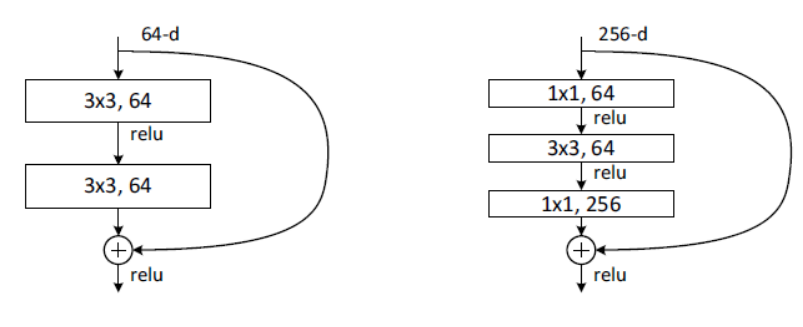
\includegraphics[width=0.60\textwidth]{png/bottleneck.png}
	\caption{Comparison of the values of European call option with default risk and European call option without default risk as $S(0)$ varies}
	\label{fig:ife1}
\end{figure}
\small
The values of European call options are shown in Table $4.1$ and Figure $4.1$, where $S(0)$ varies from $20$ to $60$, the price of European call options with default risks are evaluated by equation \eqref{eq:36} and the price of European call options without default risk, the Black-Scholes formula. Since the payoff function $(S(T)- K)^{+}$ has more probability to be large if $S(0)$ is large, the value of a European call option increases as $S(0)$ increases. This can be observed in the case of a European option with default risk, as well as European option without default risk. As shown Figure $4.1$, the value of an option with default risk is lower than one without default risk.\\
\end{frame}
\begin{frame}[allowframebreaks]
\begin{table}
\small\addtolength{\tabcolsep}{-6pt}
\begin{tabular}{c|c|c|c|c|c|c|c|c|c|c|c}
V(0) & $100$ & $120$ & $140$ & $160$ & $180$ & $200$ & $220$ & $240$ & $260$  & $280$ & $300$\\
\hline 
CBS & $8.3689$ & $8.3689$ & $8.3689$ & $8.3689$ & $8.3689$ & $8.3689$ & $8.3689$ & $8.3689$ & $8.3689$ & $8.3689$ & $8.3689$\\
\hline
C & $7.3694$ & $7.9688$ & $8.1536$ & $8.2768$ & $8.3287$ & $8.3508$ & $8.3614$ & $8.3665$ & $8.3688$ & $8.3677$ & $8.3694$\\
\end{tabular}
\caption{Values of European call option with default risk and European call option without default risk as $V(0)$ varies}
\end{table}
\small
The difference between these two derivatives due to the default risk of counterparty can be thought of as a risk premium, which is even more significant when $S(0)$ is fixed and $V(0)$ is changed as shown in Table $4.2$ and Figure $4.2$.
\end{frame}
\begin{frame}[allowframebreaks]
\begin{figure}[hp]
	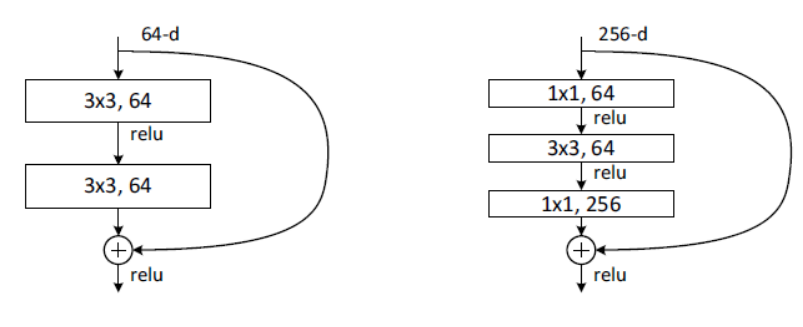
\includegraphics[width=0.60\textwidth]{png/bottleneck.png}
	\caption{Comparison of the values of European call option with default risk and European call option without default risk as $V(0)$ varies}
	\label{fig:ife2}
\end{figure}
\end{frame}
\begin{frame}[allowframebreaks]
\begin{table}
\small\addtolength{\tabcolsep}{-6pt}
\begin{tabular}{c|c|c|c|c|c|c|c|c|c|c|c}
$\sigma_{v}$ & $0$ & $0.1$ & $0.2$ & $0.3$ & $0.4$ & $0.5$ & $0.6$ & $0.7$ & $0.8$  & $0.9$ & $1$\\
\hline 
CBS & $8.3689$ & $8.3689$ & $8.3689$ & $8.3689$ & $8.3689$ & $8.3689$ & $8.3689$ & $8.3689$ & $8.3689$ & $8.3689$ & $8.3689$\\
\hline
C & $0$ & $8.0005$ & $7.3695$ & $6.7902$ & $6.337$ & $6.0072$ & $5.7689$ & $5.5933$ & $5.4637$ & $5.3655$ & $5.2896$\\
\end{tabular}
\caption{Values of European call option with default risk and European call option without default risk as $\sigma_{v}$ varies}
\end{table}
\end{frame}
\begin{frame}[allowframebreaks]
\begin{figure}[hp]
	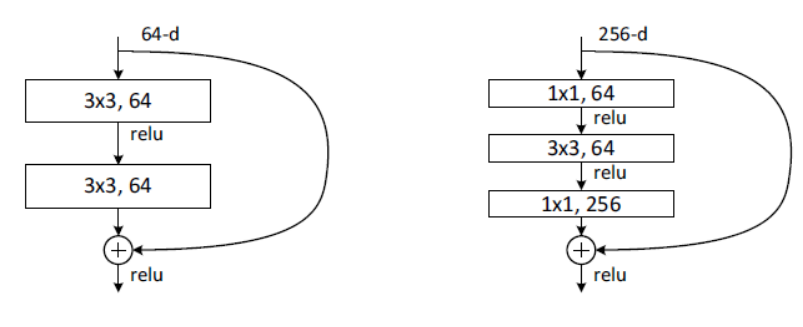
\includegraphics[width=0.60\textwidth]{png/bottleneck.png}
	\caption{Comparison of the values of European call option with default risk and European call option without default risk as $\sigma_{v}$ varies}
	\label{fig:ife3}
\end{figure}
\small
Similarly, under the same setting but different  $\sigma_{v}$ , the values of European call option with default risk and European call option without default risk also have difference which varied significantly. As shown in Table $4.3$ and Figure $4.3$, when $\sigma_{v}$ is large, ignoring the default risk of counterparty and directly using the Black-Scholes formula to assess an option with default risk will cause significant overpricing. This is due to the great default risk of counterparty when its volatility $\sigma_{v}$ is large or initial firm value $V(0)$ is too small. In contrast, when $V(0)$ is large or $\sigma_{v}$ is too small, the value of a European option with default risk tends to that of European option without default risk.
\end{frame}
\begin{frame}[allowframebreaks]
\begin{table}
\small\addtolength{\tabcolsep}{-5pt}
\begin{tabular}{c|c|c|c|c|c}
T & $1$ & $1.5$ & $2$ & $2.5$ & $3$\\
\hline 
CBS & $4.1837$ & $5.3759$ & $6.4510$ & $7.4424$ & $8.3689$\\
\hline
C & $3.766$ & $4.7952$ & $5.7292$ & $6.5797$ & $7.3695$\\
\end{tabular}
\caption{Values of European call option with default risk and European call option without default risk as T varies}
\end{table}
\end{frame}
\begin{frame}[allowframebreaks]
\begin{figure}[hp]
	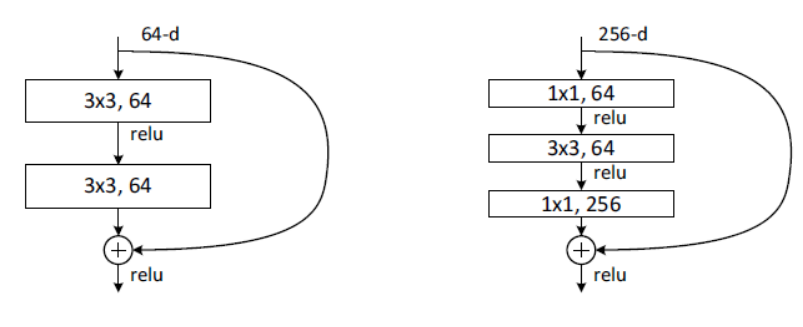
\includegraphics[width=0.60\textwidth]{png/bottleneck.png}
	\caption{Comparison of the values of European call option with default risk and European call option without default risk as $T$ varies}
	\label{fig:ife41}
\end{figure}
\small
Also, Table $4.4$ and Figure $4.4$ show the values of European call option with default risk and European call option without default risk as maturity date $T$ varies. Here, as $T$ increases, the values of European call option with default risk and European call option without default risk also increase.\\
	The black line denotes the value of European call options with default risks and the red line shows the values of European call options without default risk, evaluated by Black-Scholes formula.\\
	The above figures show that an option holder who buy the option from a small firm, in contrast to a big firm, is more vulnerable and hence needs more risk premium, which is consistent with the intuition.
\end{frame}
\small
\section{Conclusion}
\begin{frame}[allowframebreaks]{Conclusion}
In this project, we derived the analytical pricing formula for European options with default risks, releasing the constrain of default risk model used to measure the default risk of counterparty. We priced European options using the Black-Scholes model under a structural model, the first passage model which is a model for default risk. The formula for pricing European call and put options with default risks are given in equation \eqref{eq:36} and equation \eqref{eq:37}.\\ Ignoring the default risk of the counterparty, we obtained the pricing formulae of European call and put options without default risk (Black-Scholes formula) in equation \eqref{eq:38}.\\
This pricing scheme can be used to derive the pricing formula for structured notes. As example, the derivation of the value of reverse exchangeable bond is given. The numerical result was given to confirm the validity of the pricing formula. In the numerical result, the tables and figures show the values of European call options with default risk and European options without default risk as $S(0),V(0),\sigma_{v}$ and $T$ vary respectively. In figure $4.1$,it was observed that as $S(0)$ increases, the value of European call option increases. As $V(0)$ increases, the value of a European option with default risk tends to the value of a European option without default risk. Also, as $\sigma_{v}$ increases, the value of a European call option with default risk decreases. The values of European call option with default risk and European call option without default risk also increase as $T$ varies.From the result,it is clear that the price of a European option with default risk is lower than the price of a European option without default risk. 
\par The writer's assets value and underlying asset can also be modeled by a jump diffusion process.\\
Introducing a poisson process $N$ with intensity $\lambda$ under the probability measure $\mathbbm{P}$ and a sequence of independent identically distributed random variables $(U_{i})i \geq 1$ with finite expected value $\nu= \tilde{E}_{\mathbbm{P}}(U_{i})$.\\
The firm's asset value and underlying asset are given by
\begin{equation}
\label{eq:bimbo}
\frac{dV(t)}{V(t)} = (r-\lambda \nu)dt + \sigma_{v} dW_{v}(t) + d \pi(t)
\end{equation}
\begin{equation}
\label{eq:bimbola}
\frac{dS(t)}{S(t)} = (r- \lambda \nu)dt + \sigma_{s} dW_{s}(t) + d \pi(t)
\end{equation}
where $\pi$ is a jump process whose jump times are specified by the jump times of the poisson process $N$ and the $i^{th}$ jump is $U_{i}$.
$$
\pi(t) = \sum_{i=1}^{N(t)} U_{i}~\forall~t \in[0,T]
$$
\end{frame}

\begin{frame}[allowframebreaks]{References}
\bibliography{alliref}
\nocite{*}
\bibliographystyle{apacite}
\end{frame}

\begin{frame}{THANKS}
\begin{LARGE}
\textbf{THANK YOU FOR LISTENING}	
\end{LARGE}
\end{frame}
\end{document}